\documentclass{article}

\usepackage[utf8]{inputenc}

\usepackage{hyperref}

\usepackage{amsmath}

\usepackage{scrextend}

\usepackage{geometry}
\geometry{
	a4paper,
	total={170mm,257mm},
	left=20mm,
	top=20mm,
}

\usepackage{graphicx}
\usepackage[portuguese]{babel}
\usepackage{subfig}


\usepackage{listings}
\usepackage{xcolor}

\definecolor{codegreen}{rgb}{0,0.6,0}
\definecolor{codegray}{rgb}{0.5,0.5,0.5}
\definecolor{codepurple}{rgb}{0.58,0,0.82}
\definecolor{backcolour}{rgb}{0.95,0.95,0.92}

\lstdefinestyle{mystyle}{
	backgroundcolor=\color{backcolour},   
	commentstyle=\color{codegreen},
	keywordstyle=\color{magenta},
	numberstyle=\tiny\color{codegray},
	stringstyle=\color{codepurple},
	basicstyle=\ttfamily\footnotesize,
	breakatwhitespace=false,         
	breaklines=true,                 
	captionpos=b,                    
	keepspaces=true,                 
	numbers=left,                    
	numbersep=5pt,                  
	showspaces=false,                
	showstringspaces=false,
	showtabs=false,                  
	tabsize=2
}

\lstset{style=mystyle}

%\usepackage{indentfirst}
\setlength{\parindent}{1.5cm}% too much in my eyes delete this
% line and use the default ...


\title{
	Identificando transições abruptas em vídeos (trabalho 3) \\
	\Large Introdução ao Processamento de Imagem Digital \\
	Randerson A. Lemos (103897)
	2022-1S
}

\date{\vspace{-5ex}}

\begin{document}
  \pagenumbering{gobble}
  \maketitle

%
%%
\section{Introdução}
Vídeos são compostos por quadros de mesma dimensão organizados temporalmente. Esses quadros, ao serem apresentados sequencialmente (no contexto do vídeo), podem mostrar transições suaves ou abruptas. Quando presentes, essas transições abruptas entre quadros podem indicar uma sequência significativamente nova de conteúdo no vídeo e, por isso, tais transições, quando identificadas, podem ser utilizadas como material de resumo do próprio vídeo. Neste trabalho, utilizaremos quatro técnicas capazes de identificar transições abruptas entre quadros de um vídeo de acordo com certas métricas de distância. As técnicas utilizadas são: \textbf{diferenças entre pixels}; \textbf{diferenças entre blocos}; \textbf{diferenças entre histogramas}; e \textbf{diferenças entre mapas de bordas}.

%
\subsection{Diferenças entre pixels}
Aqui, para que dois quadros consecutivos sejam considerados diferentes é feita uma contagem do número de par de pixels (um de cada quadro) que são diferentes de acordo com uma tolerância $T_1$. Se essa contagem for superior a um limiar $T_2$, os quadros comparados são considerados diferentes e a transição entre eles entendida como abrupta. Tanto a tolerância $T_1$ quanto o limiar $T_2$ são parâmetros definidos pelo usuário e apresentam valores ótimos dependentes das características de cada vídeo analisado. Para o calculo da diferença entre pixels, cujo valor resultante é utilizado na comparação com a tolerância $T_1$, utiliza-se a norma 1, isto é, a diferença absoluta entre os níveis de cinza do par de pixels analisados dos quadros consecutivos.

%
\subsection{Diferenças entre blocos}
Na diferenças entre blocos é necessário subdividir os quadros consecutivos em blocos (cada quadro com seu conjunto de blocos). Feito isso, os pares de blocos correspondentes entre os quadros consecutivos são comparados e, de acordo com uma tolerância $T_1$, são ou não considerados diferentes. O número de pares de blocos entre quadros consecutivos considerados diferentes é comparado a um limiar $T_2$ e, caso esse número seja superior a tal limiar, o quadros são considerados diferentes. O blocos que subdividem os quadros possuem ou dimensão de $8x8$ ou de $16x16$. Tanto a tolerância $T_1$ quando o limiar $T_2$ são definidos pelo usuário e seus valores ótimos são dependentes das características de cada vídeo analisado.

%
\subsection{Diferenças entre histogramas}
Diferente das anteriores, nesta abordagem utilizaremos os histogramas dos quadros consecutivos, e não os valores dos pixels em si, como fonte para realização das comparações e, consequentemente, determinação de transições abruptas ou não entre tais quadros. A diferença $D_i$ entre histogramas de quadros consecutivos $i$ e $i+1$ de uma vídeo é calculada como
\[
D_i = \sum_{j=1}^{B} |H_i(j) - H_{i+1}(j)|,
\]
em que $B$ denota o número total de \textit{bins} no histograma e $H_i(j)$ é o valor do histograma para o i-ésimo quadro no nível $j$. Para avaliar se os quadros consecutivos são diferentes o suficiente para considerar que a transição correspondente seja abrupta, um limiar $T$ é calculado a partir do conjunto de todas as diferenças $D_i$ obtidas. Em posse da média $\mu$ e do desvio padrão $\sigma$ das diferenças $D_i$ o limiar $T$ é obtido pela equação
\[
T = \mu + \alpha\sigma,
\]
em que $\alpha$ é definido pelo usuário. Ao parâmetro $alpha$ é atribuído valores típicos entre $3$ e $6$.¨

%
\subsection{Diferenças entre bordas}
Na diferenças entre bordas, utiliza-se o mapa de bordas dos quadros consecutivos como fonte de informação para determinação ou não de uma transição abrupta entre esses quadros. A abordagem adotada para verificação da diferença entre quadros consecutivos foi a contagem do número de pixels das bordas de cada quadro seguida da subtração absoluta desses valores. O número resultante dessa operação é comparado com um limiar $T$. Caso tal número seja superior que esse limiar, os quadros são considerados diferentes e a transição correspondente abrupta. 
%
%%
\section{Solução}
A solução utiliza a linguagem de programação Python e conta com o auxílio do gerenciador de projetos e pacotes Conda. Assumindo que o usuário tenha o Conda instalado em sua máquina, a configuração do projeto pode ser feita pela execução do comando \lstinline{conda env create -f environment.yml} a partir da pasta do projeto \textbf{trab3}. Esse comando cria o ambiente de trabalho \textbf{mc920-trab3} e instala os seguintes módulos: opencv, numpy, scipy, pandas, matplotlib. Finalizada a configuração do ambiente de trabalho em questão, o usuário deve executar o comando \lstinline{source source.sh}\footnote{O comando que configura o ambiente de trabalho mc920-trab3 precisa ser executado apenas um vez. Assim sendo, depois que este ambiente está configurado, o usuário precisa apenas executar o comando \lstinline{source source.sh}} para carregar as variáveis de ambiente adequadas e, assim, poder usar os programas do projeto dentro do próprio ambiente de trabalho recém configurado. 

Dos arquivos presentes na pasta do projeto \textbf{trab3}, destacam-se as pastas \textbf{assets}, \textbf{classes}, \textbf{tex} e o programa \textbf{main.py}. A pasta \textbf{assets} contém vídeos no formato png ou mpg que podem ser utilizados para a aplicação das técnicas de identificação de transições abruptas implementadas. A pasta \textbf{classes} contém arquivos com as implementações das diferentes técnicas de identificação de transições abruptas em formato de classes. Os arquivos das classes das técnicas são: \textbf{blocksdifferences.py}, \textbf{edgesdifferences.py}, \textbf{histogramdifferences.py}, e \textbf{pixelsdifferences.py}. A pasta \textbf{tex} contém os arquivos Latex deste relatório. O programa \textbf{main.py} contém as implementações necessárias para aplicar as técnicas de identificação de transições abruptas no vídeo de entrada fornecido pelo usuário. Informações pertinentes das implementações serão apresentadas a seguir.

%
\subsection{Main.py}
O programa \textbf{main.py} é responsável pela aplicação de todas as técnicas consideradas de identificação de transições abruptas entre quadros consecutivos de vídeos. Para ser executado, esse programa precisa receber o parâmetro de entrada \textbf{video\_entrada}:

\begin{itemize}
	\item ao parâmetro \textbf{video\_entrada} deve-se fornecer o nome do arquivo do vídeo a ser utilizado para aplicação das técnicas de identificação de transições abruptas.
\end{itemize}
	
\noindent 
O programa \textbf{main.py} disponibiliza tanto um vídeo no formato $mp4$ dos quadros considerados como pertencentes a transições abruptas como também gráficos em formato png da evolução dos valores de distância utilizados para determinação de transições abruptas ou não. Todo esse conteúdo é salvo dentro da pasta \textbf{out} que está localizada dentro da pasta do projeto \textbf{trab3}.

Um exemplo de como executar o programa \textbf{main.py} utilizando os recursos contidos dentro do próprio projeto é: \lstinline{python3 main.py -video_entrada=assets/lisa.mpg}.

O programa \textbf{main.py} executa quatro funções principais, as quais são: \textbf{main\_pixels\_differences( path, stem )}; \textbf{main\_blocks\_differences( path, stem )}; \textbf{main\_histog\_differences( path, stem )}; e \textbf{main\_edges\_differences( path, stem )}. Cada uma dessas funções é responsável por executar a técnica de identificação de transições abruptas que encapsula várias vezes utilizando diferentes combinações de parâmetros de entrada (tolerâncias e limiares). Essas funções também estão encarregadas de salvar todo o conteúdo gerado (os vídeos e gráficos) com nomes intuitivos dentro da pasta \textbf{out}. A seguir olharemos para essas funções e, principalmente, para as técnicas de identificação de transições abruptas associadas.


%
\subsection{main\_pixels\_differences( path, stem )}
Esse função roda a classe \textbf{PixelsDifferences} sobre as tuplas resultantes do produto cartesiano entre os conjuntos $MPNDS \times MPNNS$ cujos elementos são
\[
MPNDS = \{0.1; 0.2; 0.3; 0.4; 0.5; 0.6; 0.7 \}
\]
e
\[
MPNNS = \{0.1; 0.2; 0.3; 0.4; 0.5; 0.6; 0.7 \}.
\]
MPNDS é sigla de \textit{Maximum Pixel Normalized Distances} e MPNNS é sigla de \textit{Maximum Pixel Normalized Numbers}. Os valores do conjunto MPNDS fazem referência a tolerância $T_1$ utilizada para verificar se dois pixels são ou não significativamente diferentes. Os valores do conjunto NPNNS fazem referência ao limiar $T_2$, que é utilizado para determinar se o número final de pixels considerados diferentes é suficiente para que os quadros consecutivos sejam classificados como tendo uma transição abrupta. Ambos os valores dos conjuntos em questão apresentam domínio pertencente ao intervalo $[0,1]$ porque tanto o calculo da tolerância $T_1$ quando do limiar $T_2$ e feito de maneira normalizada. Para comparação com a tolerância $T_1$, o cômputo da distância entre pixels é feita da seguinte maneira
\[
	d_{xy} = | Q_i(x,y) - Q_{i+1}(x,y) | / 255,
\]
em que $Q_i(x,y)$ é o valor de intensidade do pixel da posição $(x,y)$ do i-ésimo quadro em escala de cinza do vídeo analisado. Como a diferença máxima entre pixels em escala de cinza representados com 1 bite é de 255, o valor da variável $d$ sempre vai pertencer ao intervalo $[0,1]$. Para comparação com o limiar $T_2$ o cômputo do numero de pixels que apresentam transições abruptas é feita assim
\[
D_i = \sum_{x=0}^{x=M}\sum_{y=0}^{y=N} (1 \text{  se  } d_{xy} > T_1 \text{  caso contrario  } 0.
\]
Caso $D_i$, isto é o número de pixels considerados diferentes de acordo com a tolerância $T_1$ entre o i-ésimo e (i+1)-ésimo quadros, for superior que o limiar $T_2$, o quadro (i+1)-ésimo é classificado como contendo uma transição abrupta.


%
\subsection{main\_blocks\_differences( path, stem )}
Esse função roda a classe \textbf{BlocksDifferences} sobre as tuplas resultantes do produto cartesiano entre os conjuntos $MBNDS \times MBNNS$ cujos elementos são
\[
MBNDS = \{0.1; 0.2; 0.3; 0.4; 0.5; 0.6; 0.7 \}
\]
e
\[
MBNNS = \{0.1; 0.2; 0.3; 0.4; 0.5; 0.6; 0.7 \}.
\]
MBNDS é sigla de \textit{Maximum Block Normalized Distances} e MBNNS é sigla de \textit{Maximum Block Normalized Numbers}. Os valores do conjunto MBNDS fazem referência a tolerância $T_1$ utilizada para verificar se dois blocos são ou não significativamente diferentes. Os valores do conjunto NBNNS fazem referência ao limiar $T_2$, que é utilizado para determinar se o número final de blocos considerados diferentes é suficiente para que os quadros consecutivos sejam classificados como tendo uma transição abrupta. Ambos os valores dos conjuntos em questão apresentam domínio pertencente ao intervalo $[0,1]$ porque tanto o calculo da tolerância $T_1$ quando do limiar $T_2$ e feito de maneira normalizada. 

Para comparação com a tolerância $T_1$ o cômputo da distância entre blocos é feita da seguinte maneira
\[
d_ai = \sum_{w=0}^{8}\sum_{k=0}^{8}(B_{a_{i}}(w,k) - B_{a_{i+1}}(w,k))^2 / 255^2,
\]
em que $d_ai$ é a distância quadrática normalizada dos a-ésimos blocos entre os quadros $i$ e $i+1$. Logo $B_{a_{i}}(w,k)$ é o valor em escala de cinza do pixel que está na posição $(w,k)$ do a-ésimo bloco da i-ésima imagem. Os valores de $d_ai$ estão contidos no intervalo $[0,1]$ (o termo $255^2$ é um fator de normalização). 

Para comparação com o limiar $T_2$, o número total de blocos que violam a tolerância $T_1$ é levantado e, se esse valor ultrapassar o limiar $T_2$, os quadros consecutivos utilizados na comparação por meio dos seus blocos são considerados como possuidores de transições abruptas. Os valore utilizados em $T_2$ estão normalizados pelo número total de blocos que cabe nos quadros do vídeo analisado e por isso também estão contidos dentro do intervalo $[0,1]$.
%
\subsubsection{Detalhes de implementação e execução}
Como requisitado no trabalho, a classe \textbf{BlocksDifferences} é capaz de trabalhar com blocos de $8\times8$ ou $16\times16$. No entanto para os resultados mostrados, apenas execuções com blocos de tamanho $8\times8$ foram considerados. Sobre o problema do casamento exato ou não entre as dimensões dos blocos (que pode ser de $8\times8$ ou $16\times16$) e as dimensões da imagem o tratamento dado foi: Começar sempre a subdivisão da imagem em blocos a partir da posição $(0,0)$ e, caso ocorra, as possíveis bordas presentes na parte da direita ou na parte de baixo da imagem são desconsideradas.


%
\subsection{main\_histog\_differences( path, stem )}
Esse função roda a classe \textbf{HistogramDifferences} sobre o conjunto dos valores
\[
\alpha = \{3,4,5,6\},
\]
que são os valores sugeridos na descrição do trabalho. Nenhuma modificação na forma de se calcular a diferença dos histogramas de quadros consecutivos foi realizada de modo que tal cálculo já está explicitado na parte da secção de introdução que trata desse técnica de identificação de mudanças abruptas entre quadros. No entanto vale destacar que os histogramas foram normalizados de modo que a soma dos valores de seus \textit{bins} totaliza 1.
%
\subsubsection{Detalhes de implementação e execução}
Para o cálculo dos histogramas, optou-se por utilizar uma implementação própria ao invés de usar alguma função disponibilizada pelos módulos do opencv ou do numpy.


%
\subsection{main\_edges\_differences( path, stem )}
Essa função roda a classe \textbf{EdgesDifferences} sobre o conjuto de valores
\[
    MENDS = [0.010, 0.015, 0.020, 0.025, 0.030, 0.035].
\]
MENDS é sigla de \textit{Maximum Edges Normalized Difference}. Os valores desse conjunto estão dentro do itervalo $[0,1]$ e eles representam a diferença máxima normalizada de bordas entre quadros consecutivos tolerada. A normalização é feita considerando a diferença máxima de bordas entre quadros consecutivos possível que ocorreria quando um quadro não teria nenhuma borda e o outro quadro teria apenas `bordas'. Logo a diferença máxima possível, nessa situação, seria igual ao número de pixels dos quadros do vídeo analisado.


%
\subsubsection{Detalhes de implementação e execução}
Para o cálculo do mapa de bordas, foi utilizado o famoso algoritmo Canny que foi desenvolvido por John F. Canny. Esse algoritmo é bastante popular devido a sua versatilidade e robustez. Ele contempla etapas de redução de ruídos, determinação das intensidades do gradiente da imagem, e aplicação de supressão não máxima e teste de hipóteses. Utilizou-se a versão do algoritmo disponibilizada pelo módulo do opencv $Canny$ com os parâmetros de entrada fixos. O parâmetro de valor mínimo de 100 e o parâmetro de valor máximo de 200. 

Mesmo o algoritmo de detecção de bordas de Canny já conter um etapa de suavização de ruídos, optou-se antes de aplicá-lo, suavizar o quadro de interesse bom um filtro Gaussiano (passa-baixo) de dimensão $5\times5$.


\section{Resultado}
Todos os resultados apresentados foram gerados pelo processamento do vídeo \textbf{lisa.mpg} que está dentro da pasta \textbf{assets}. Devido ao grande número de combinações de parâmetros das quatro técnicas de identificação de mudanças abruptas entre quadros considerados e, consequentemente, o grade número de conteúdo gerado (entre vídeos e gráficos) serão apresentados aqui apenas um subconjunto desses materiais (caso haja interesse do leitor em verificar a totalidade desse conteúdo basta acessá-los dentro da pasta \textbf{out}). Aquim, serão apresentados os gráficos gerados que evidenciam o quão diferentes são dois quadros consecutivos e o número de quadros que foram considerados como detenedores de uma transição abrupta.

\newpage
\subsection{Diferenças entre pixels}

\begin{figure}[!htp]%
	\centering
	\subfloat[\centering Gráfico dos quadros com trasições abruptas para $T_1=0.1$ e $T_2=0.1$ (veja vídeo: \url{https://youtu.be/BLa\_RR3D7Hw}).]{{ 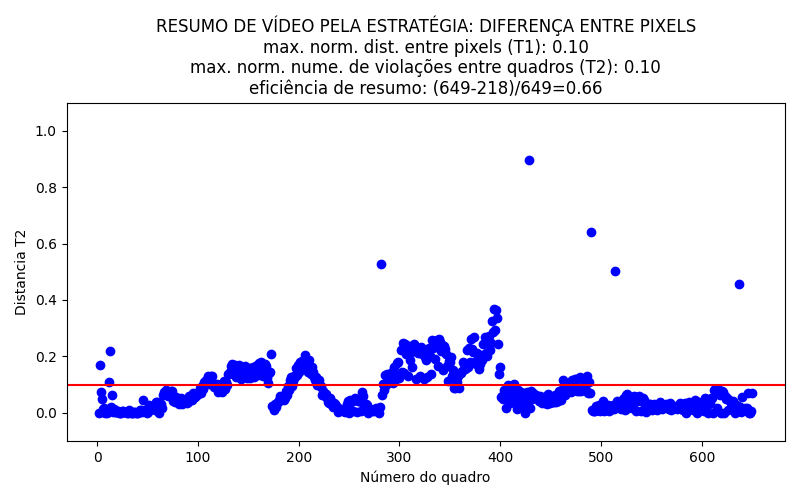
\includegraphics[width=10cm]{lisa_pixeldiff_mpnd_10_mpnn_10_nframe_00218.png} 
	}}%
	\\
	\subfloat[\centering Gráfico dos quadros com trasições abruptas para $T_1=0.1$ e $T_2=0.3$ (veja vídeo: \url{https://youtu.be/dqFbqMDnW90}).]{{ 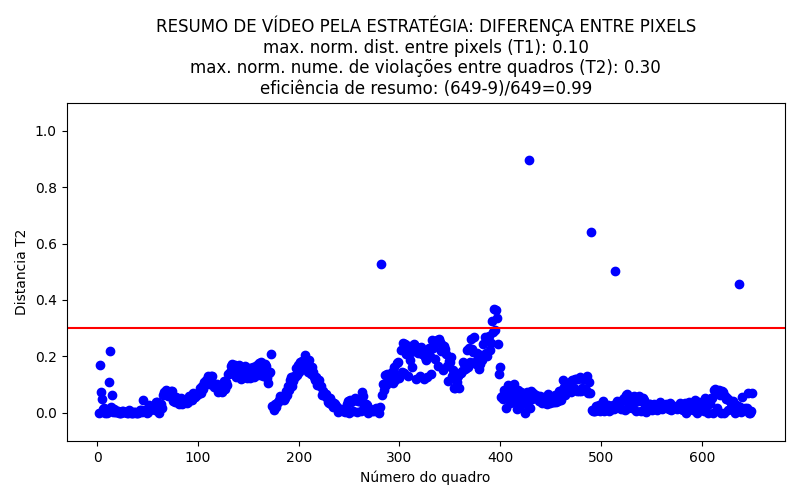
\includegraphics[width=10cm]{lisa_pixeldiff_mpnd_10_mpnn_30_nframe_00009.png} 
	}}%	
	\\
	\subfloat[\centering Gráfico dos quadros com trasições abruptas para $T_1=0.1$ e $T_2=0.5$ (veja vídeo: \url{https://youtu.be/9uXixvLlcV4}).]{{ 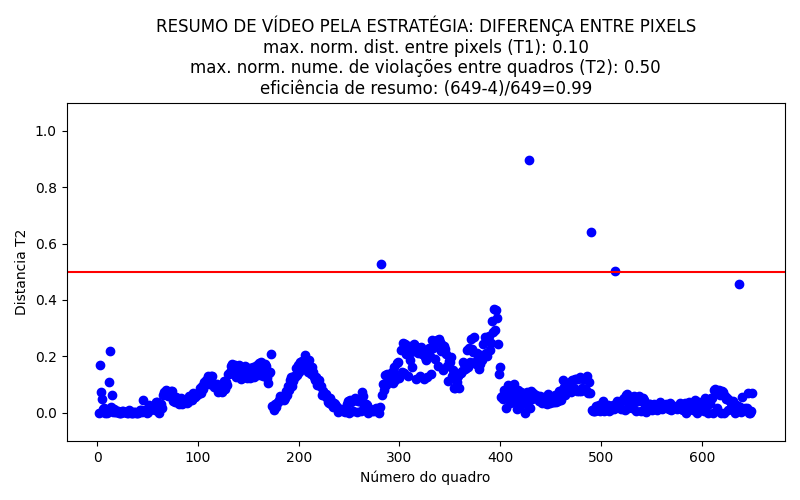
\includegraphics[width=10cm]{lisa_pixeldiff_mpnd_10_mpnn_50_nframe_00004.png} 
	}}%	
	\caption{Imagem com gráficos do número de pixels (distância do limiar $T_2$) com diferenças de valores entre quadros consecutivos superiores a tolerância $T_1$.}%	
	\label{fig:diferenca_pixels}%
\end{figure}

\newpage
\subsection{Diferenças entre blocos}

\begin{figure}[!htp]%
	\centering
	\subfloat[\centering Gráfico dos quadros com trasições abruptas para $T_1=0.4$ e $T_2=0.1$ (veja vídeo: \url{https://youtu.be/mm43T9BhlUU}).]{{ 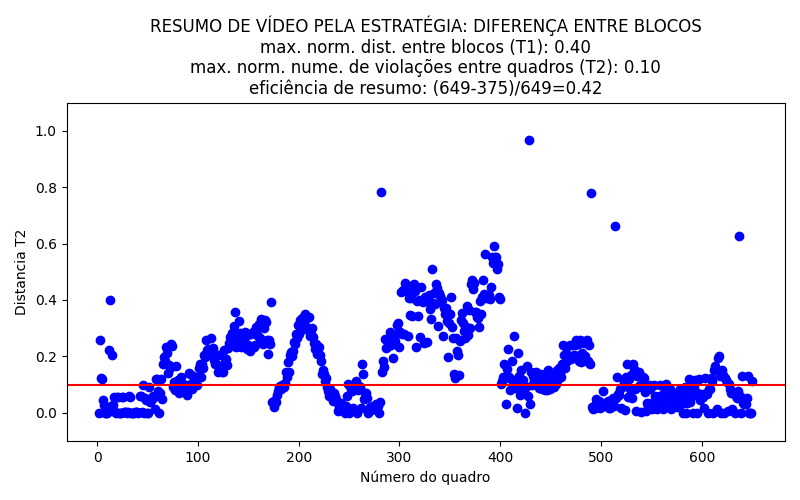
\includegraphics[width=10cm]{lisa_blockdiff_mbnd_40_mbnn_10_nframe_00375.png} 
	}}%
	\\
	\subfloat[\centering Gráfico dos quadros com trasições abruptas para $T_1=0.4$ e $T_2=0.3$ (veja vídeo: \url{https://youtu.be/r4TxG6zJtIg}).]{{ 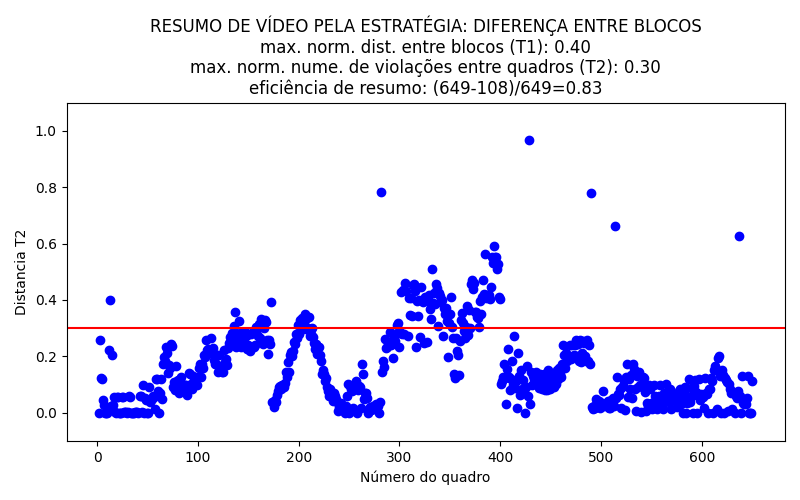
\includegraphics[width=10cm]{lisa_blockdiff_mbnd_40_mbnn_30_nframe_00108.png} 
	}}%	
	\\
	\subfloat[\centering Gráfico dos quadros com trasições abruptas para $T_1=0.4$ e $T_2=0.5$ (veja vídeo: \url{https://youtu.be/5yxTwq2srKw}).]{{ 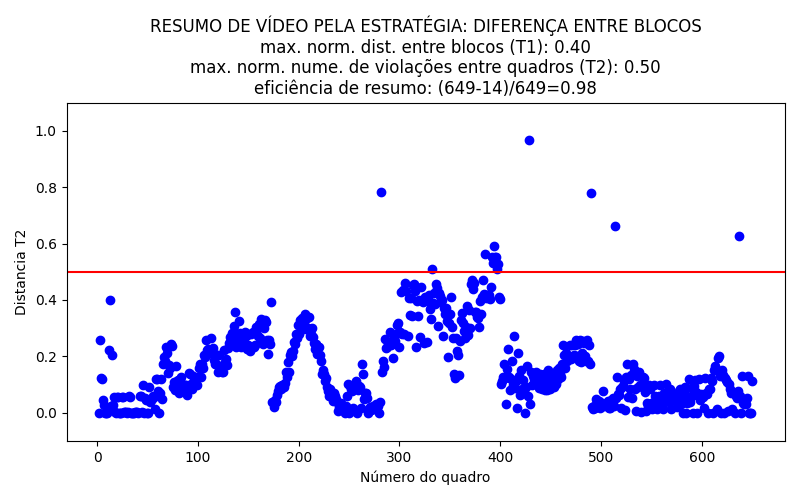
\includegraphics[width=10cm]{lisa_blockdiff_mbnd_40_mbnn_50_nframe_00014.png} 
	}}%	
	\caption{Imagem com gráficos do número de blocos (distância do limiar $T_2$) com diferenças de valores entre quadros consecutivos superiores a tolerância $T_1$.}%	
	\label{fig:diferenca_blocos}%
\end{figure}


\newpage
\subsection{Diferenças entre histograma}

\begin{figure}[!htp]%
	\centering
	\subfloat[\centering Gráfico dos quadros com trasições abruptas para $\alpha=3$ (veja vídeo: \url{https://youtu.be/taISwMqDRO4}).]{{ 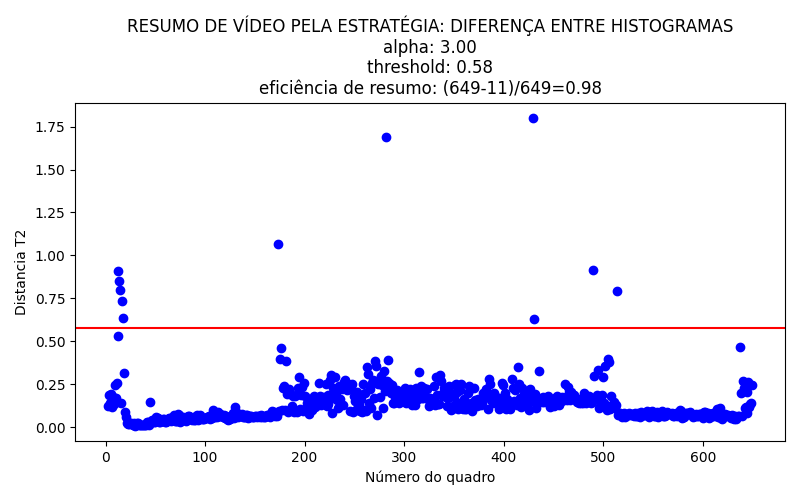
\includegraphics[width=10cm]{lisa_histdiff_alpha_3_thres_0.578_nframe_00011.png} 
	}}%
	\\
	\subfloat[\centering Gráfico dos quadros com trasições abruptas para $\alpha=4$ (veja vídeo: \url{https://youtu.be/hoMm_-U1uqY}).]{{ 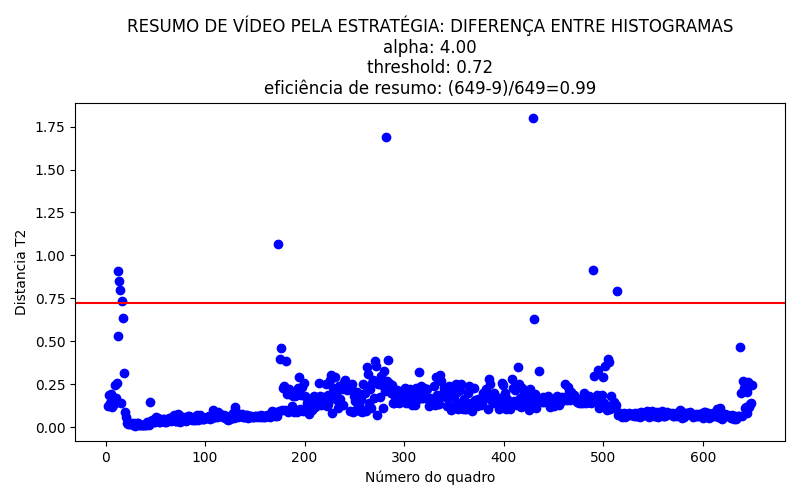
\includegraphics[width=10cm]{lisa_histdiff_alpha_4_thres_0.723_nframe_00009.png} 
	}}%	
	\\
	\subfloat[\centering Gráfico dos quadros com trasições abruptas para $\alpha=5$ (veja vídeo: \url{https://youtu.be/-NX1KpQSwvM}).]{{ 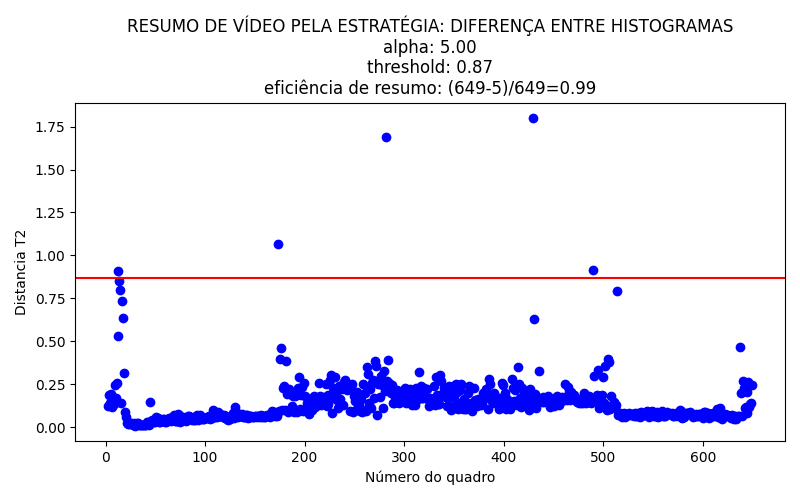
\includegraphics[width=10cm]{lisa_histdiff_alpha_5_thres_0.867_nframe_00005.png} 
	}}%	
	\caption{Imagem com gráficos da diferença entre quadro consecutivos por meio da técnica da diferença entre histogramas.}%	
	\label{fig:diferenca_histogramas}%
\end{figure}


\newpage
\subsection{Diferenças entre borda}

\begin{figure}[!htp]%
	\centering
	\subfloat[\centering Gráfico dos quadros com trasições abruptas para $T=0.01$ (veja vídeo: \url{https://youtu.be/OpjOwV45uxY}).]{{ 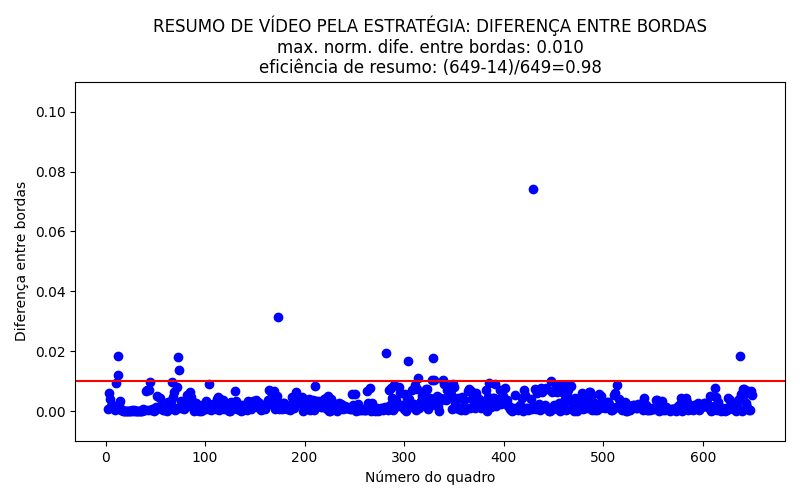
\includegraphics[width=10cm]{lisa_edgediff_mpnd_1.0_nframe_00014.png} 
	}}%
	\\
	\subfloat[\centering Gráfico dos quadros com trasições abruptas para $T=0.015$ (veja vídeo: \url{https://youtu.be/ICLpevnXpGE}).]{{ 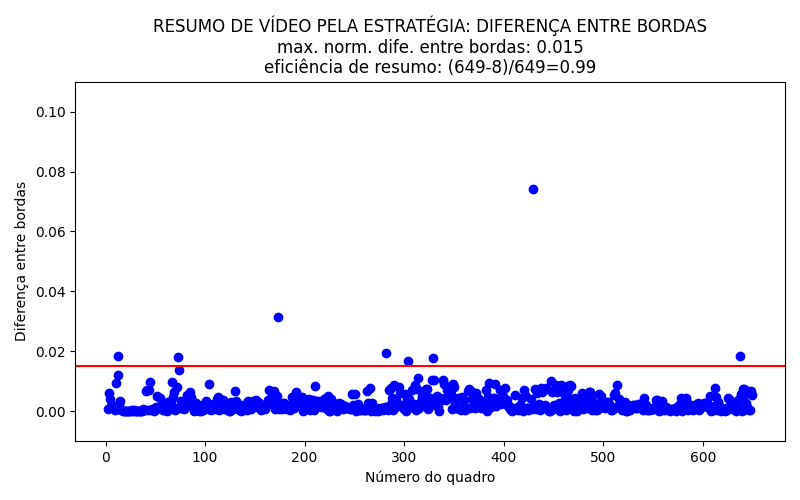
\includegraphics[width=10cm]{lisa_edgediff_mpnd_1.5_nframe_00008.png} 
	}}%	
	\\
	\subfloat[\centering Gráfico dos quadros com trasições abruptas para $T=0.02$ (veja vídeo: \url{https://youtu.be/Qkp-s1RcZSM}).]{{ 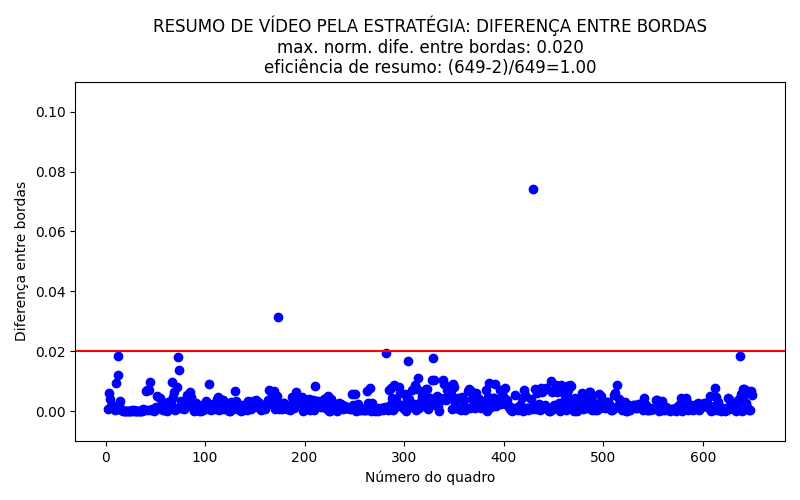
\includegraphics[width=10cm]{lisa_edgediff_mpnd_2.0_nframe_00002.png} 
	}}%	
	\caption{Imagem com gráficos da diferença entre quadro consecutivos por meio da técnica da diferenças entre borda.}%	
	\label{fig:diferenca_bordas}%
\end{figure}
%
%%
\section{Discussão e Conclusão}
É possível verificar, dos gráficos apresentados, que as diferentes técnicas de identificação de transições abruptas discriminam os quadros consecutivos de maneira significativamente diferente. Esse afirmação se sustenta pelos diferentes padrões de distribuição dos valores do eixo y ao longo do eixo x. Nesse aspecto (dos padrões de descriminação), há uma aproximação entre os comportamentos das técnicas de diferenças entre pixel e diferenças entre bloco (Figuras \ref{fig:diferenca_pixels} e \ref{fig:diferenca_blocos}) e entre os comportamentos das técnicas de diferenças entre histograma e diferenças entre borda (Figuras \ref{fig:diferenca_histogramas} e \ref{fig:diferenca_bordas})). Percebe-se que as técnicas de diferenças entre pixel e diferenças entre borda apresentam maior dificuldade em discriminar os quadros consecutivos com transições abruptas que as técnicas de diferenças entre histograma e de diferenças entre borda já que nas duas primeiras técnicas há maior amplitude nos valores de distância do eixo y que nas duas últimas técnicas.

Por outro lado, as técnicas de diferenças entre pixel e diferenças entre borda se mostraram menos custosas em termos computacionais que as técnicas de diferenças entre histograma e diferenças entre borda.

É também facilmente verificável que o desempenho das técnicas, no sentido de encontrar uma quantidade aceitável de quadros significativos, é  intimamente relacionado com os valores dos seus parâmetros. Por exemplo, na técnica de diferença entre blocos encontrou-se para os parâmetros $T_1=0.40$ e $T_2=0.10$ o número de $375$ quadros significativos de um total de $649$ quadros (um resultado pouco animador). No entanto, essa mesma técnicas, para os valores de parâmetros $T_1=0.40$ e $T_2=0.50$, encontrou um total de $14$ quadros com transições abruptas de uma total de $649$ quadros (um resultado bem mais interessante) (Figura \ref{fig:diferenca_blocos}).

Para o vídeo utilizado nesse trabalho, as técnicas de diferenças entre histograma e diferenças entre borda se mostraram mais interessantes. Essas técnicas encontraram um conjunto significativamente pequeno de quadros com transições abruptas (afirmação que pode ser comprovada visualizando os vídeos disponibilizados no youtube). Para a técnica de diferenças entre histograma com a configuração de $\alpha=5$ foram encontrados 5 quadros significativos (com transições abruptas) )(Figura \ref{fig:diferenca_histogramas}). Já para a técnica de diferenças entre bordas para $T=0.015$ (Figura \ref{fig:diferenca_bordas}), foram encontrados 8 quadros com transições abruptas. Esses números são bastante impressionantes e trazem uma eficiência de redução de vídeos de aproximadamente $99\%$.

Do apresentado, podemos verificar que as técnicas (umas melhores que outras) foram capazes de identificar quadros associados a transições abruptas do vídeo analisado. 

Caso haja necessidade de uma solução de identificação de transições abruptas entre quadros consecutivos mais robusta, uma alternativa seria experimentar o desempenho de um técnica resultante da combinação linear das técnicas aqui implementadas. Por fim, a técnicas foram satisfatoriamente implementadas e testadas.
\end{document}
